\chapter{Onderzoeks plan}\label{ch:onderzoekPlan}


\section{Inleiding en aanleiding}\label{sec:inleiding-en-aanleiding}% TODO: Wellicht weglaten en inleiding kaal laten beginnen
% todo: opnieuw schrijven
In het vorige hoofdstuk~\ref{ch:opdracht} is de opdracht voor dit onderzoek duidelijk uitgeschreven. In dit hoofdstuk wordt uitgewijd over hoe deze opdracht wordt onderzocht met als resultaat een methode die geimplementeerd kan worden.
[NOTE:]Gezien de te ontwikkelen module een zekere impact zal hebben op de manier van werken binnen EagleScience is het goed om een solide plan van aanpak te hebben voor er daadwerkelijk begonnen wordt aan het ontwikkelen en uitrollen van de module. Hieronder worden de vershillende fasen van het project beschreven met daarbij de geschatte tijd die het gaat duren. Het project vangt aan in september 2021 aan en de oplevering van de module is gepland voor wordt gezet op eind januari 2022. Om hieraan te kunnen voldoen moeten er een aantal milestones worden gedefinieerd. Hieronder volgt een globale beschrijving van de milestones, opleveringen, en methodes die gebruikt worden om de milestone te halen.


\section{Probleemanalyse}\label{sec:probleemanalyse}
Eaglescience heeft de ambitie om te groeien in zowel het aantal projecten dat het aanneemt als in het personeelsaantal. Daarnaast is het bezig met het integreren van het software lifecycle management paradigma in het kwaliteitssysteem om zo een gerichte-, transparante en traceerbare aanpak te hebben over de kwaliteit en daarmee dus ook de veiligheid van de software die geleverd wordt. Om deze redenen wordt er gezocht naar manieren om taken die veel voorkomen en bijdragen aan de kwaliteit te automatiseren om op die manier een traceerbare en transparante aanpak te hebben. Eén van de taken die geautomatiseerd moet worden is het analyseren van externe applicatie componenten\footnote{componenten die gebruikt worden om een applicatie op te bouwen, gedacht kan worden aan: operatingSystems, Ontwikkeltalen, bibliotheken en frameworks. ( dit onderzoek gaat voornamelijk over externe bibliotheken en frameworks)}, en dan met name de biblioteken en frameworks. Ook wel Software of Unkown Provenance (SOUP) genoemd.

Deze soup analyses worden nu geheel met de hand gedaan door een ontwikkelaar van een project en heeft als resultaat een document in confluence met de bevindingen. Na de analyse dienen de componenten die out-of-date en/of bewezen kwetsbaarheden bevatten geupdate worden. Dit proces dient gezien de complexiteit van de projecten ook na een geautomatiseerde oplossing met de hand gedaan te worden. Doordat de Analyse met de hand wordt gedaan dient deze ingeplanned te worden bij een ontwikkelaar die op zijn beurt hier tijd aan moet besteden die niet altijd door de klant betaald kan worden, vaak door SLA-afspraken. Onder andere om deze reden wordt deze analyse minder vaak uitgevoerd dan gewenst.

%Probleem stelling
Het probleem is dus dat de in de huidige vorm van een SOUP-analyse veel tijd zit die anders besteed kan worden. Daarnaast wordt de analyse niet frequent genoeg gedaan en veelal op momenten wanneer deze inplanbaar is. En daarom de probleemstelling: "Ontwikkel een methode die automatisch en periodiek een SOUP-analuse doet op de projecten die EagleScience in haar beheer heeft".

De probleemstelling geeft de volgende Centrale vraag: "Welke methode is het meest geschikt voor het geautomatiseerd en periodiek uitvoeren van een SOUP analyse voor alle in beheer zijn projecten binnen EagleScience


\section{Doelstellingen}\label{sec:doelstellingen}
Het doel van dit onderzoek is inzicht krijgen in methodes om een SOUP analyse te doen binnen de dev-stack van EagleScience. Hierbij moet rekening gehouden worden met de in de opdracht gegeven criteria. Waarvan de belangrijkste is dat er zo min mogelijke impact moet zijn op de huidige werkwijze die op dit moment gehanteerd wordt.
%TODO: uitbreiden en anders samenvoegen met probleemstelling


%TODO: Checken of de stakeholders analyse wel in dit deel moet komen. of toch in een eigen deel van het ontwerp.


\section{Stakeholdersanalyse}\label{sec:stakeholdersanalyse}
Binnen EagleScience zijn er een aatal stakeholders die belang hebben bij deze een uitkomst van dit onderzoek en daarmee een nieuwe methode/module voor een SOUP-analyse. Naast de stakeholders binnen Eaglescience is er nog een stakeholder in de vorm van de klant. Hoewel de klant niet actief is in de ontwikkeling van deze methode/module, hebben zij wel degelijk belang bij het resultaat en dienen dan ook genoemd te worden.

\subsection{Dagelijks bestuur (intern)}\label{subsec:dagelijks-bestuur-(intern)1}
Het dagelijks bestuur ziet vooral voordelen in het inzicht krijgen van kwetsbaarheden op een overzichtelijke manier, zodat ze kunnen sturen in het gebruik van biblioteken of andere technologiën. Ook al zullen er kosten die niet direct terug te verdienen zijn gemoeit met de ontwikkeling van een nieuwe methode.
Echter, zien zij ook kosten gemoeid met de verandering.
Door de manier van werken dienen deze kosten terug verdient te worden door werkzaamheden binnen andere projecten.
De CTO ziet vooral tijdswinst zodat de time-to-market voor andere projecten hoger ligt en dus meer verdient kan worden.

\subsection{Projectmanagers (intern)}\label{subsec:projectmanagers-(intern)1}
Project managers krijgen op dit moment een update over de staat van kwetsbaarheden tijdens stand-ups en aan het einde van een sprint tijdens de sprint demo's.
De nieuwe module biedt ze de mogelijkheid om up-to-date informatie on-demand te verkrijgen.
Op de vraag of het het waard is dat een aantal ontwikkelaars tijd kwijt zijn in testen en meedenken over de module weegt volgens hen op tegen de voordelen die de module in de toekomst kan brengen.

\subsection{Ontwikkelteam (intern)}\label{subsec:ontwikkelteam-(intern)1}
Het ontwikkelteam wil graag meedenken en meewerken aan een oplossing, gezien zij de gene waren die handmatig de analyse uitvoerden.
Zij zien voor een oplossing voor een taak dat veel tijd in beslag nam en afleide van de daadwerkelijke taak.

\subsection{Klant (extern)}\label{subsec:klant-(extern)1}
Als laatste de klant welke een passieve stakeholder is gezien zij niet direct betrokken zijn bij de ontwikkeling van de module maar wel verbeteringen genieten in de zin van veilige en betrouwbare software.

\subsection{Stakeholder analyse}\label{subsec:stakeholder-analyse1}
\begin{figure}[H]
    \myfloatalign
    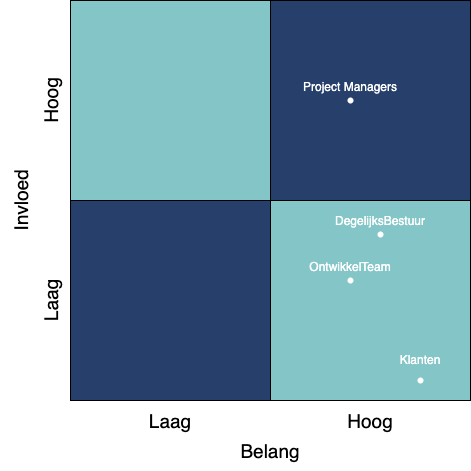
\includegraphics[width=10cm]{gfx/stakeholderanalyse}
    \caption{StakeHolders Analyse}
    \label{fig:StakeholderAnalyse1}
\end{figure}
[NOTE]Figuur stakeholder analyse nog aanpassen.
Zoals te zien is in figuur~\ref{fig:StakeholderAnalyse1} zijn de projectmanager, het ontwikkelteam en de klanten het meest gebaad bij een nieuwe module voor de analyse van kwetsbaarheden.
Echter zijn de klanten niet tot bijna niet betrokken bij de ontwikkeling van de module maar hebben er indirect wel belang bij omdat de software die voor hen ontwikkeld wordt veiliger wordt door het voeren van een geautomatiseerde analyse.
Door deze analyse worden alleen de requirements meegnomen die intern zijn opgenomen.


\section{Theoretisch kader}\label{sec:theoretisch-kader}

Het theoretisch kader waarmee gewerkt wordt bestaat uit twee hoofdelen. Het eerste hoofddeel is de werkwijze EagleScience en de gebruikte technologiën. De Bronnen die hiervoor gebruikt zijn zijn de volgende:
\begin{itemize}
    \item \textbf{151030 F04B Proces Flow Chart ES\_V1.0\_TN.pdf} een document dat de workflow beschrijft die binnen EagleScience gehanteerd wordt.
    \item \textbf{200121\_Policy Manual\_ES\_V6 signed.pdf} ISO handboek waarin de bedrijfsvoering binnen EagleScience wordt beschreven.
\end{itemize}
Deze documenten geven een basis over de werkwijze van EagleScience. En zal dus als input gelden voor het ontwerp dat plaats gaat vinden na het onderzoek.
Het tweede hoofddeel is de theorie omtrent externe bibliotheken, het gebruik en daarmee de potentiële gevaren hiervan en methoden om deze bibliotheken te analyseren. Als ingangspunt is de OWASP Top-10 gekozen omdat de inhoud van dit document binnen EagleScience geldt als aandachtspunten voor het ontwikkelen van veilige software. De basis voor dit onderzoek wordt beschreven in punt "A06:2021-Vulnerable and Outdated Components" waarin beschreven wordt welke gevaren er potentieel dreigen als op dit punt niets gedaan wordt. Andere bronnen zijn:
\begin{itemize}
    \item \textbf{Justifying the use of software of uncertain pedigree (SOUP) in safety-related applications} P.G.\ Bishop, R.E.\ Bloomfield and P.K.D.\  Froome for Adelard 2001. Hoewel dit document verouderd lijkt staat er wel degelijk intressante informatie over waarom je SOUP zou gebruiken en hoe je de risico's kan verminderen.
    \item \textbf{Backstabber’s Knife Collection: A Review of Open Source Software Supply Chain Attacks} Marc Ohm, Henrik Plate, Arnold Sykosch, and Michael Meier: 2020: Dit artikel bevat informatie over een mogelijke vorm van aanvallen die middels SOUP uitgevoerd zouden kunnen worden. Daarnaast geeft het artikel inzicht in hoe de onderzoekers packages voor NPM, Python, en Ruby hebben onderzocht.
    \item \textbf{https://www.owasp.org}Naast de bovenstaande artikelen is de website van OWASP een bron van informatie op het gebied van tooling en methodes. ()
\end{itemize}
Het Laatste hoofdeel bestaat uit de resultaten van de bovengenoemde onderdelen waarmee een voor eaglescience geschikte methode wordt gevonden. Naast de resultaten van de twee voorgaande hoofdelen worden de volgende bronnen geraadpleegd als leidraad voor het ontwerp:
\begin{itemize}
    \item \textbf{System Analysis \& Design An Object-Oriented Approach with UML 5th Edition}Alan Dennis, Barbara Haley Wixom, David Tegarden: Boek over het ontwerp van software in het algemeen de hoofdstukken over requirements analyse en gathering zijn veel gebruikt in het onderzoek.
    \item
\end{itemize}
\newpage
\section{Conceptueel model}\label{sec:conceptueel-model}
Om de verschillende onderzoeken in goed banen te leiden is er een conceptueel model opgesteld die de relaties van de verschillende onderzoeken waarborgt.
\begin{figure}[H]
    \centering
    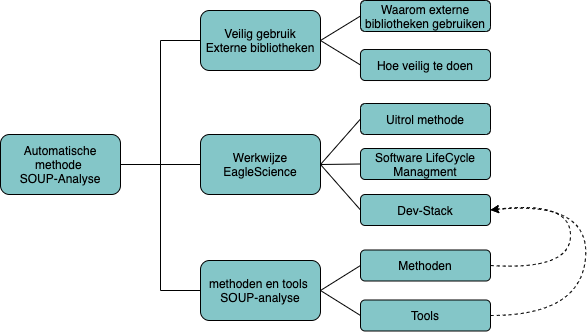
\includegraphics[width=10cm]{gfx/Conceptueel Model}
    \caption{Conceptueel Model}
    \label{fig:ConceptueelModel}
\end{figure}

In figuur~\ref{fig:ConceptueelModel} is het conceptueel model opgenomen dat voor deze opdracht is opgesteld. Dit model maakt de samenhang van de verschillende begrippen duidelijk.

Het kernbegrip is "Automatische methode SOUP analyse" en staat voor het eind conclussie die het onderzoek moet opleveren in de zin van een conclussie over tools en een methode die gebruikt kunnen worden in het ontwerp van de module. Om tot deze conclussie te komen zijn er vier begrippen die ieders een eigen domein binnen de probleemstelling belichten. Zo zal "werkwijze EagleScience" de manier van werken binnen Eaglescience belichten als ook de manier van uitrollen en de dev-stack die gebruikt gaat worden. Ook komt hier de Software Lifecycle Managment aan bod gezien dit één van de aanleidingen voor de opdracht. Het theoretische deel van het onderzoek wordt onderzocht in "veilig gebruik externe bibliotheken" waarin wordt gekeken waarom er bibliotheken van buitenaf worden gebruikt en wat de potentiële gevaren zijn die dit met zich meebrengt. Het begrip methoden en tools zal ingaan op de beschikbare tools die gebruikt kunnen worden om een analyse te doen. Met deze tools wordt een methode onderzocht die het mogelijk maakt met de constraints die EagleScience heeft om een SOUP analyse te doen. Met als resultaaat een theoretische methode die als input kan gelden voor het ontwerp voor de nieuwe module die in de opdracht staat beschreven. Deze nieuwe module dient in de EagleScience Portal opgenomen te worden en om die reden is het begrip "Huidig architctuur EagleScience Portal" waarin wordt onderzocht hoe de portal ontworpen is en welke dev-stack er is gebruikt.

\section{Deelvragen}\label{sec:deelvragen}
Aan de hand van het theoretisch kader, conceptueel model en de doelstellingen zijn er de volgende deelvragen voor dit onderzoek opgesteld:
\textbf{Dev-stack binnen Eaglescience}
\begin{itemize}
    \item hoe wordt binnen EagleScience het software lifecycle management paradigma ingevoerd?
    \item Welk proces wordt er binnen Eaglescience gebruikt om software te ontwikkelen en hoe resulteert dit is een dagelijkse werkwijze?
    \item Wat zijn de meest gebruikte ontwikkeltalen en frameworks die binnen EagleScience worden toegepast?
    \item Welke tooling wordt er gebruikt binnen EagleScience? [NOTE relevant?]
    \item Hoe wordt er binnen EagleScience software uitgerold?
\end{itemize}
\textbf{Theorie over SOUP}
\begin{itemize}
    \item Wat is veilige software?
    \item Wat is SOUP?
    \item Wat dragen externe bibliotheken en dus ook potentieel SOUP bij aan de ontwikkeling van software?
    \item Wat zijn de gevaren van het gebruik van SOUP?
    \item Wordt er ergens bijgehouden of een dependency/component) een kwetsbaaheid bevat?
    \item Wat relateert SOUP tot software veiligheid binnen EagleScience?
\end{itemize}
\textbf{Methodes om een SOUP analyse te doen binnen de Dev-stack van EagleScience}
\begin{itemize}
    \item Welke tools bestaan er om dependency informatie uit een sbt en npm project te halen?
    \item Hoe zijn de tools in te zetten in de huidige projecten?
    \item Welke output wordt er verkregen van de tools?
    \item Welke manieren zijn er om uit de huidige pipeline informatie over de deploy te halen?
    \item Wat zijn hier de voor en nadelen van?
\end{itemize}


\section{Onderzoeksontwerp}\label{sec:onderzoeksontwerp}
Gezien de grote hoeveelheid deelvragen die benoemd zijn op basis van de onderzoeksvraag en het conceptueel model is het verstandig om het onderzoek in kleinere onderzoeken te verdelen. Door het op te delen in deelonderzoeken kan het kader beter worden vastgesteld en zal er minder snel "teveel" worden onderzocht. De deel onderzoeken zal op de volgende manier worden opgesplitst:
\begin{enumerate}
    \item \textbf{Werkwijze en dev-stack Eaglescience} Dit onderzoek moet inzicht geven in de dagelijkse manier van werken binnen EagleScience en de daarbij gebruikte dev-stack. Het resultaat is inzicht in hoe EagleScience applicaties ontwikkeld en hoe deze uitgerold wordt. Daarnaast is er inzicht in hoe er op dit moment een SOUP analyse wordt gedaan.
    \item \textbf{Theorie SOUP analyses} Om een methode te kunnen ontwikkelen is er een theoretische basis nodig. Dit onderzoek geeft inzicht in de theoretische basis en het belang om een analyse te doen. Daarnaast wordt er uitgezocht hoe er het beste een analyse gedaan kan worden.
    \item \textbf{Methode voor Soup analyse binnen EagleSciende} Door inzichten uit voorgaande onderzoeken te combineren en nieuwe kennis toe te voegen is er een ontwerp voor een implementatie die aan de opdracht voldoet.
\end{enumerate}

\subsection{strategie}\label{subsec:opstrategie}
Om de drie onderzoeken die hierboven beschreven zijn goed uit te kunnen voeren zijn er de volgende strategien bedacht die ervoor zorgen dat er een betrouwbaar resultaat is waar verder mee gewerkt kan worden.
Voor het onderzoek binnen de huidige situatie binnen EagleScience wordt interne documentatie geraadpleegd aangevuld met vraag gesprekken met collega's die met het onderwerp te maken hebben. Deze gespreken zullen worden gehouden in delen gezien de manier waarop er binnen EagleScience gewerkt wordt. (heeft te maken met het aantal niet declarabele uren die ieder persoon wel of niet heeft). Het onderzoek naar de theorie van SOUP analyses wordt uitgevoerd middels een deskresearch waarbij in literatuur gezocht wordt naar methoden om de analyse te doen. Daarnaast wordt er een selectie gemaakt in tools die al ontwikkeld zijn die bruikbaar zijn voor het einddoel van de opdracht. In het laatste onderzoek wordt gekeken naar een method die past bij de huidige manier van werken binnen eaglescience, en de tools die gevonden zijn. Ook wordt er een ontwerp gemaakt hoe de methode eruit komt te zien er welke data dit oplevert waarna er een module ontwikkeld kan worden die deze data inzichtelijk maakt voor de stakeholders.

\section{planning}\label{sec:planning}
Om tijdig tot resultaten te komen is de volgende planning.

\subsection{Requirements analyse \textbf{september 2021}}\label{subsec:requirements-analyse}
Na het ontvangen van de opdracht dient er onderzocht te worden of er naast de eisen die door de CTO in de opdracht zijn gezet nog andere eisen zijn binnen EagleScience. Hiervoor zal er onderzocht worden welke betrokkenen er zijn en welke belangen en wensen zij hebben. Na het houden van interviews zullen alle wensen tegen elkaar worden afgewogen. Dit zal leiden tot een document waarin alle belangrijke requirements worden geprioriteerd volgens de MoSCoW\-methode.

\textbf{Methode:} Intake gesprek met opdrachtgever, interviews met betrokkenen, enquete voor ontwikkelaars.

\textbf{Resultaat:} Applicatie requirements document.

\subsection{Vooronderzoek \textbf{september 2021 - oktober 2021 }}\label{subsec:onderzoek}
Om de requirements om te kunnen zetten naar een ontwerp zal er onderzoek gedaan worden naar de huidige manier van ontwikkelen en compileren van de software. Een onderzoek naar begrippen binnen het domein SOUP is een voorwaarde om vervolgens onderzoek te kunnen doen naar methodes om analyses te kunnen doen op software die EagleScience maakt ten opzichte van SOUP. De resultaten van het vooronderzoek zullen worden gebruikt als input.
Om meer kennis en verdieping te krijgen in de materie rondom de nieuwe module zullen er een aantal onderzoeken worden uitgevoerd.


Er is onderzoek nodig naar de volgende onderwerpen:
\begin{itemize}
    \item \textbf{Architectuur binnen EagleScience} Werkwijze en ontwikkel stack van EagleScience met daarin specifiek onderzocht hoe er omgegaan wordt met het voorkomen van onveiligheden in de geleverde software
    \item \textbf{Externe bibliotheken gebruik en het gevaar} Onderzoek naar waarom er externe bibliotheken worden gebruikt en het gevaar hiervan.
    \item \textbf{Soup Analyse} Door te kijken naar de kwetsbaarheden in de externe bibliotheken kan er beter worden nagegaan of er kwetsbaarheden in de software zitten. Dit onderzoek zal in gaan op het bestaan van methodes om SOUP analyses te doen. En een mogelijkheid om dit (deels) geautomatiseerde te doen.
\end{itemize}

\textbf{Methode:} Bureau onderzoek, interviews met specialisten, meedoen aan en/of terugkijken van conferenties

\textbf{Resultaat:} Inzicht in het begrip SOUP en software veiligheid als ook een idee voor een mogelijke implementatie van de oplossing die voor EagleScience de beste is zonder veel impact op de huidige manier van werken te hebben.

\subsection{Initieel ontwerp \textbf{oktober 2021 - november 2021 }}\label{subsec:initieel-ontwerp}
Er zal een ontwerp worden gemaakt waarin vast gelegd is welke requirements er beslist in de module moeten zitten en de uitwerking van deze. Evenals een ontwerp van de architectuur en het datamodel. Naast de module zal er ook een ontwerp gemaakt worden voor een ontwikkel/test omgeving om de module continue te kunnen testen zonder dat dit de huidige buildstraat beinvloed. Dit laatste is van belang om zo min mogelijk storingen te veroorzaken in de dagelijkse gang van zaken bij al lopende projecten. Het eerste ontwerp zal als leidraad dienen voor de implementatie waarin afgeweken kan worden als dit nodig blijkt tijdens de implementatie sprints.

\textbf{Methode:} Overleggen met ontwikkelaars, huidige omgeving onderzoeken op mogelijkheden en architectuur.
\textit{wellicht nog toevoegen als resultaten: blokdiagram van oplossing/architectuur; sequence diagram om te komen van analyse tot rapportage (er is een handig tooltje om deze diagrammen te tekenen: https://bramp.github.io/js-sequence-diagrams/)}
\textbf{Resultaat:} Eerste ontwerp in de vorm van een datamodel, blokdiagram van architectuur voor de oplossing, als ook een sequence diagram om van analyse tot rapportage te komen.

\textit{4.4: Gebruik hier of de template ontwikkel omgeving voor (aparte branch/taak); of de portal ontwikkelomgeving
4.4: Voeg rij resultaat toe: klaar voor review of gereviewde}

\subsection{Implementatie en Testen \textbf{november 2021 - januari 2022 }}\label{subsec:implementatie-en-testen}
Om te kunnen beginnen aan de implementatie is er een ontwikkel/ test omgeving nodig die het mogelijk maakt om zonder invloed op de dagelijkse werkzaamheden van EagleScience een module te kunnen ontwikkelen. Deze zal eerst worden opgezet. Als test projecten zullen snapshots worden gebruikt van de daadwerkelijke projecten dit om een zo accuraat mogelijke test omgeving te hebben. Zoals in de opdracht beschreven dient de nieuwe module een onderdeel te zijn van de bestaande portal. Er zal dan ook direct samen worden gewerkt met het team die daar op het moment mee aan het ontwikkelen is. Tijdens de implementatie zal er ook worden gedocumenteerd wordt hoe de module werkt en welke procedures hier in worden gevolgd. Dit document biedt ontwikkelaars de mogelijkheid om dit door te nemen als on-boarding en referentie.

\textbf{Methode:} Agile scrum sprints met iedere 2 weken een oplevermoment en demo als ook een reflectie op de sprint.
\textbf{Resultaat:} Werkende en geteste applicatie die klaar is om uitgerold te worden.

\subsection{Uitrollen en documentatie \textbf{januari 2022 - februari 2022 }}\label{subsec:uitrollen-en-documentatie}
Nadat de implementatie van de meest kritische requirements is afgerond zal er worden begonnen met het uitrollen van de module en het testen door een geselecteerde groep gebruikers. De feedback wordt bekeken en meegenomen in de evaluatie. Mocht het nodig zijn dan zal er accuut actie worden ondernomen om deze wijzigingen aan te passen. Mochten er wensen zijn die kunnen wachten dan zal er worden overwogen om deze mee te nemen in de volgende iteratie van het project. (de verwachting is dat de module die hier beschreven wordt verder zal worden uitgebreid met de diverse mogelijkheden om betere en veiligere software te ontwikkelen.) Daarnaast zal ook de documentatie verder worden afgerond.
\textbf{Methode:} Interviews met stakeholders met een analyse over de nieuwe requirements.

\textbf{Resultaat:} Uitegrolde en gedocumenteerde applicatie
